\section{Test environment for ClickHouse performance tests}
\label{app:ch-perf}
Azure CLI commands were run in the Azure Cloud Shell (PowerShell).

Bash commands (the commands run on the VM) were run as \texttt{azureuser}
(the default user) in \path{/home/azureuser}, unless specified otherwise.

SQL queries were run in \texttt{clickhouse-client}.

The VM used had the following specifications:
\begin{itemize}
\item 16 GB of RAM
\item 4 vCPUs
\item 2048GB SSD
\item Ubuntu 16.04
\end{itemize}

The procedure for setting the environment up is generally the same as for the normal test environment
(see [cref]).

\subsection{Declare variables}
\label{sec:org306c306}
The following variables were declared to make scripts more reusable.
They are mostly the same as the normal test environment,
except having ``perf'' (performance) prefixed.

\begin{minted}[breaklines=true,breakanywhere=true]{powershell}
$AzCloudUser = "torstein"        # Name of Azure user used for CLI commands
$RGName = "perfRG"               # Name of resource group
$CHName = "perfClickhouseVM"         # Name of VM running ClickHouse
$SSHKey = "mySSHKey"             # Name of SSH key used to connect to VM
$SSHPath = "/home/$AzCloudUser/.ssh/$SSHKey.pub"  # Path of SSH keys in Azure Cloud Shell storage
$SAName = "perfchbksa"               # Name of storage account used by clickhouse-backup
$ContainerName = "chbkperfcontainer" # Name of container storing clickhouse-backup data
$StagingSAName = "perfstagingchsa"   # Name of storage account used for Azure Backup staging
$SASExpDate = "2022-05-18"       # Expiry date of SAS token used by clickhouse-backup
$location = "eastus"             # Location of Azure resources
$RSVName = "perfRSV"               # Name of Recovery Services Vault
$subscription = "4b48eb85-91f3-4902-b74b-e84641fb6785"  # Subscription ID
$PolicyName = "DefaultPolicy"    # Policy to be used by Azure Backup
\end{minted}
\subsection{Set up a resource group}
\label{sec:orgccc1bce}
Create resource group:
\begin{minted}[breaklines=true,breakanywhere=true]{powershell}
az group create --name $RGName --location $location
\end{minted}

Output:
\begin{minted}[breaklines=true,breakanywhere=true]{json}
{
  "id": "/subscriptions/4b48eb85-91f3-4902-b74b-e84641fb6785/resourceGroups/perfRG",
  "location": "eastus",
  "managedBy": null,
  "name": "perfRG",
  "properties": {
    "provisioningState": "Succeeded"
  },
  "tags": null,
  "type": "Microsoft.Resources/resourceGroups"
}
\end{minted}
\subsection{Set up a VM}
\label{sec:orgc560500}
Create an Ubuntu VM:
\begin{minted}[breaklines=true,breakanywhere=true]{powershell}
az vm create `
    --resource-group $RGName `
    --name $CHName `
    --image Canonical:UbuntuServer:16.04-LTS:16.04.202109280 `
    --admin-username azureuser `
    --size Standard_D4s_v4 `
    --os-disk-size-gb 2048 `
    --ssh-key-values $SSHPath `
    --public-ip-sku Standard
\end{minted}

Output:
\begin{minted}[breaklines=true,breakanywhere=true]{json}
{
  "fqdns": "",
  "id": "/subscriptions/4b48eb85-91f3-4902-b74b-e84641fb6785/resourceGroups/perfRG/providers/Microsoft.Compute/virtualMachines/perfClickhouseVM",
  "location": "eastus",
  "macAddress": "00-22-48-25-AA-BE",
  "powerState": "VM running",
  "privateIpAddress": "10.0.0.4",
  "publicIpAddress": "20.237.81.139",
  "resourceGroup": "perfRG",
  "zones": ""
}
\end{minted}
\subsection{Install ClickHouse}
\label{sec:org963a40c}
Commands to install ClickHouse were copied from the installation guide in the ClickHouse documentation [InstallationClickHouseDocs].
The ClickHouse default user password was left empty.

\begin{minted}[breaklines=true,breakanywhere=true]{bash}
sudo apt-get install -y apt-transport-https ca-certificates dirmngr
sudo apt-key adv --keyserver hkp://keyserver.ubuntu.com:80 --recv 8919F6BD2B48D754

echo "deb https://packages.clickhouse.com/deb stable main" | sudo tee \
    /etc/apt/sources.list.d/clickhouse.list
sudo apt-get update

sudo apt-get install -y clickhouse-server clickhouse-client

sudo service clickhouse-server start
\end{minted}

\subsection{Load test data}
\label{sec:orgf169474}
Followed instructions at
[\url{https://ghe.clickhouse.tech/}]

The compressed size was 200GB when loaded in the database.
The dataset was therefore loaded 5 times into different tables in ClickHouse,
in order to fill the database with 1TB of compressed data.

Commands were run on the VM.

Install tool for decompression:
\begin{minted}[breaklines=true,breakanywhere=true]{bash}
sudo apt install pixz
\end{minted}

Download compressed dataset:
\begin{minted}[breaklines=true,breakanywhere=true]{bash}
wget https://datasets.clickhouse.com/github_events_v2.native.xz
\end{minted}

Create five tables for the data in \texttt{clickhouse-client}:
\begin{minted}[breaklines=true,breakanywhere=true]{sql}
CREATE TABLE github_events1
(
    file_time DateTime,
    event_type Enum('CommitCommentEvent' = 1, 'CreateEvent' = 2, 'DeleteEvent' = 3, 'ForkEvent' = 4,
                    'GollumEvent' = 5, 'IssueCommentEvent' = 6, 'IssuesEvent' = 7, 'MemberEvent' = 8,
                    'PublicEvent' = 9, 'PullRequestEvent' = 10, 'PullRequestReviewCommentEvent' = 11,
                    'PushEvent' = 12, 'ReleaseEvent' = 13, 'SponsorshipEvent' = 14, 'WatchEvent' = 15,
                    'GistEvent' = 16, 'FollowEvent' = 17, 'DownloadEvent' = 18, 'PullRequestReviewEvent' = 19,
                    'ForkApplyEvent' = 20, 'Event' = 21, 'TeamAddEvent' = 22),
    actor_login LowCardinality(String),
    repo_name LowCardinality(String),
    created_at DateTime,
    updated_at DateTime,
    action Enum('none' = 0, 'created' = 1, 'added' = 2, 'edited' = 3, 'deleted' = 4, 'opened' = 5, 'closed' = 6, 'reopened' = 7, 'assigned' = 8, 'unassigned' = 9,
                'labeled' = 10, 'unlabeled' = 11, 'review_requested' = 12, 'review_request_removed' = 13, 'synchronize' = 14, 'started' = 15, 'published' = 16, 'update' = 17, 'create' = 18, 'fork' = 19, 'merged' = 20),
    comment_id UInt64,
    body String,
    path String,
    position Int32,
    line Int32,
    ref LowCardinality(String),
    ref_type Enum('none' = 0, 'branch' = 1, 'tag' = 2, 'repository' = 3, 'unknown' = 4),
    creator_user_login LowCardinality(String),
    number UInt32,
    title String,
    labels Array(LowCardinality(String)),
    state Enum('none' = 0, 'open' = 1, 'closed' = 2),
    locked UInt8,
    assignee LowCardinality(String),
    assignees Array(LowCardinality(String)),
    comments UInt32,
    author_association Enum('NONE' = 0, 'CONTRIBUTOR' = 1, 'OWNER' = 2, 'COLLABORATOR' = 3, 'MEMBER' = 4, 'MANNEQUIN' = 5),
    closed_at DateTime,
    merged_at DateTime,
    merge_commit_sha String,
    requested_reviewers Array(LowCardinality(String)),
    requested_teams Array(LowCardinality(String)),
    head_ref LowCardinality(String),
    head_sha String,
    base_ref LowCardinality(String),
    base_sha String,
    merged UInt8,
    mergeable UInt8,
    rebaseable UInt8,
    mergeable_state Enum('unknown' = 0, 'dirty' = 1, 'clean' = 2, 'unstable' = 3, 'draft' = 4),
    merged_by LowCardinality(String),
    review_comments UInt32,
    maintainer_can_modify UInt8,
    commits UInt32,
    additions UInt32,
    deletions UInt32,
    changed_files UInt32,
    diff_hunk String,
    original_position UInt32,
    commit_id String,
    original_commit_id String,
    push_size UInt32,
    push_distinct_size UInt32,
    member_login LowCardinality(String),
    release_tag_name String,
    release_name String,
    review_state Enum('none' = 0, 'approved' = 1, 'changes_requested' = 2, 'commented' = 3, 'dismissed' = 4, 'pending' = 5)
)
ENGINE = MergeTree
ORDER BY (event_type, repo_name, created_at)

CREATE TABLE github_events2
(
    file_time DateTime,
    event_type Enum('CommitCommentEvent' = 1, 'CreateEvent' = 2, 'DeleteEvent' = 3, 'ForkEvent' = 4,
                    'GollumEvent' = 5, 'IssueCommentEvent' = 6, 'IssuesEvent' = 7, 'MemberEvent' = 8,
                    'PublicEvent' = 9, 'PullRequestEvent' = 10, 'PullRequestReviewCommentEvent' = 11,
                    'PushEvent' = 12, 'ReleaseEvent' = 13, 'SponsorshipEvent' = 14, 'WatchEvent' = 15,
                    'GistEvent' = 16, 'FollowEvent' = 17, 'DownloadEvent' = 18, 'PullRequestReviewEvent' = 19,
                    'ForkApplyEvent' = 20, 'Event' = 21, 'TeamAddEvent' = 22),
    actor_login LowCardinality(String),
    repo_name LowCardinality(String),
    created_at DateTime,
    updated_at DateTime,
    action Enum('none' = 0, 'created' = 1, 'added' = 2, 'edited' = 3, 'deleted' = 4, 'opened' = 5, 'closed' = 6, 'reopened' = 7, 'assigned' = 8, 'unassigned' = 9,
                'labeled' = 10, 'unlabeled' = 11, 'review_requested' = 12, 'review_request_removed' = 13, 'synchronize' = 14, 'started' = 15, 'published' = 16, 'update' = 17, 'create' = 18, 'fork' = 19, 'merged' = 20),
    comment_id UInt64,
    body String,
    path String,
    position Int32,
    line Int32,
    ref LowCardinality(String),
    ref_type Enum('none' = 0, 'branch' = 1, 'tag' = 2, 'repository' = 3, 'unknown' = 4),
    creator_user_login LowCardinality(String),
    number UInt32,
    title String,
    labels Array(LowCardinality(String)),
    state Enum('none' = 0, 'open' = 1, 'closed' = 2),
    locked UInt8,
    assignee LowCardinality(String),
    assignees Array(LowCardinality(String)),
    comments UInt32,
    author_association Enum('NONE' = 0, 'CONTRIBUTOR' = 1, 'OWNER' = 2, 'COLLABORATOR' = 3, 'MEMBER' = 4, 'MANNEQUIN' = 5),
    closed_at DateTime,
    merged_at DateTime,
    merge_commit_sha String,
    requested_reviewers Array(LowCardinality(String)),
    requested_teams Array(LowCardinality(String)),
    head_ref LowCardinality(String),
    head_sha String,
    base_ref LowCardinality(String),
    base_sha String,
    merged UInt8,
    mergeable UInt8,
    rebaseable UInt8,
    mergeable_state Enum('unknown' = 0, 'dirty' = 1, 'clean' = 2, 'unstable' = 3, 'draft' = 4),
    merged_by LowCardinality(String),
    review_comments UInt32,
    maintainer_can_modify UInt8,
    commits UInt32,
    additions UInt32,
    deletions UInt32,
    changed_files UInt32,
    diff_hunk String,
    original_position UInt32,
    commit_id String,
    original_commit_id String,
    push_size UInt32,
    push_distinct_size UInt32,
    member_login LowCardinality(String),
    release_tag_name String,
    release_name String,
    review_state Enum('none' = 0, 'approved' = 1, 'changes_requested' = 2, 'commented' = 3, 'dismissed' = 4, 'pending' = 5)
)
ENGINE = MergeTree
ORDER BY (event_type, repo_name, created_at)

CREATE TABLE github_events3
(
    file_time DateTime,
    event_type Enum('CommitCommentEvent' = 1, 'CreateEvent' = 2, 'DeleteEvent' = 3, 'ForkEvent' = 4,
                    'GollumEvent' = 5, 'IssueCommentEvent' = 6, 'IssuesEvent' = 7, 'MemberEvent' = 8,
                    'PublicEvent' = 9, 'PullRequestEvent' = 10, 'PullRequestReviewCommentEvent' = 11,
                    'PushEvent' = 12, 'ReleaseEvent' = 13, 'SponsorshipEvent' = 14, 'WatchEvent' = 15,
                    'GistEvent' = 16, 'FollowEvent' = 17, 'DownloadEvent' = 18, 'PullRequestReviewEvent' = 19,
                    'ForkApplyEvent' = 20, 'Event' = 21, 'TeamAddEvent' = 22),
    actor_login LowCardinality(String),
    repo_name LowCardinality(String),
    created_at DateTime,
    updated_at DateTime,
    action Enum('none' = 0, 'created' = 1, 'added' = 2, 'edited' = 3, 'deleted' = 4, 'opened' = 5, 'closed' = 6, 'reopened' = 7, 'assigned' = 8, 'unassigned' = 9,
                'labeled' = 10, 'unlabeled' = 11, 'review_requested' = 12, 'review_request_removed' = 13, 'synchronize' = 14, 'started' = 15, 'published' = 16, 'update' = 17, 'create' = 18, 'fork' = 19, 'merged' = 20),
    comment_id UInt64,
    body String,
    path String,
    position Int32,
    line Int32,
    ref LowCardinality(String),
    ref_type Enum('none' = 0, 'branch' = 1, 'tag' = 2, 'repository' = 3, 'unknown' = 4),
    creator_user_login LowCardinality(String),
    number UInt32,
    title String,
    labels Array(LowCardinality(String)),
    state Enum('none' = 0, 'open' = 1, 'closed' = 2),
    locked UInt8,
    assignee LowCardinality(String),
    assignees Array(LowCardinality(String)),
    comments UInt32,
    author_association Enum('NONE' = 0, 'CONTRIBUTOR' = 1, 'OWNER' = 2, 'COLLABORATOR' = 3, 'MEMBER' = 4, 'MANNEQUIN' = 5),
    closed_at DateTime,
    merged_at DateTime,
    merge_commit_sha String,
    requested_reviewers Array(LowCardinality(String)),
    requested_teams Array(LowCardinality(String)),
    head_ref LowCardinality(String),
    head_sha String,
    base_ref LowCardinality(String),
    base_sha String,
    merged UInt8,
    mergeable UInt8,
    rebaseable UInt8,
    mergeable_state Enum('unknown' = 0, 'dirty' = 1, 'clean' = 2, 'unstable' = 3, 'draft' = 4),
    merged_by LowCardinality(String),
    review_comments UInt32,
    maintainer_can_modify UInt8,
    commits UInt32,
    additions UInt32,
    deletions UInt32,
    changed_files UInt32,
    diff_hunk String,
    original_position UInt32,
    commit_id String,
    original_commit_id String,
    push_size UInt32,
    push_distinct_size UInt32,
    member_login LowCardinality(String),
    release_tag_name String,
    release_name String,
    review_state Enum('none' = 0, 'approved' = 1, 'changes_requested' = 2, 'commented' = 3, 'dismissed' = 4, 'pending' = 5)
)
ENGINE = MergeTree
ORDER BY (event_type, repo_name, created_at)

CREATE TABLE github_events4
(
    file_time DateTime,
    event_type Enum('CommitCommentEvent' = 1, 'CreateEvent' = 2, 'DeleteEvent' = 3, 'ForkEvent' = 4,
                    'GollumEvent' = 5, 'IssueCommentEvent' = 6, 'IssuesEvent' = 7, 'MemberEvent' = 8,
                    'PublicEvent' = 9, 'PullRequestEvent' = 10, 'PullRequestReviewCommentEvent' = 11,
                    'PushEvent' = 12, 'ReleaseEvent' = 13, 'SponsorshipEvent' = 14, 'WatchEvent' = 15,
                    'GistEvent' = 16, 'FollowEvent' = 17, 'DownloadEvent' = 18, 'PullRequestReviewEvent' = 19,
                    'ForkApplyEvent' = 20, 'Event' = 21, 'TeamAddEvent' = 22),
    actor_login LowCardinality(String),
    repo_name LowCardinality(String),
    created_at DateTime,
    updated_at DateTime,
    action Enum('none' = 0, 'created' = 1, 'added' = 2, 'edited' = 3, 'deleted' = 4, 'opened' = 5, 'closed' = 6, 'reopened' = 7, 'assigned' = 8, 'unassigned' = 9,
                'labeled' = 10, 'unlabeled' = 11, 'review_requested' = 12, 'review_request_removed' = 13, 'synchronize' = 14, 'started' = 15, 'published' = 16, 'update' = 17, 'create' = 18, 'fork' = 19, 'merged' = 20),
    comment_id UInt64,
    body String,
    path String,
    position Int32,
    line Int32,
    ref LowCardinality(String),
    ref_type Enum('none' = 0, 'branch' = 1, 'tag' = 2, 'repository' = 3, 'unknown' = 4),
    creator_user_login LowCardinality(String),
    number UInt32,
    title String,
    labels Array(LowCardinality(String)),
    state Enum('none' = 0, 'open' = 1, 'closed' = 2),
    locked UInt8,
    assignee LowCardinality(String),
    assignees Array(LowCardinality(String)),
    comments UInt32,
    author_association Enum('NONE' = 0, 'CONTRIBUTOR' = 1, 'OWNER' = 2, 'COLLABORATOR' = 3, 'MEMBER' = 4, 'MANNEQUIN' = 5),
    closed_at DateTime,
    merged_at DateTime,
    merge_commit_sha String,
    requested_reviewers Array(LowCardinality(String)),
    requested_teams Array(LowCardinality(String)),
    head_ref LowCardinality(String),
    head_sha String,
    base_ref LowCardinality(String),
    base_sha String,
    merged UInt8,
    mergeable UInt8,
    rebaseable UInt8,
    mergeable_state Enum('unknown' = 0, 'dirty' = 1, 'clean' = 2, 'unstable' = 3, 'draft' = 4),
    merged_by LowCardinality(String),
    review_comments UInt32,
    maintainer_can_modify UInt8,
    commits UInt32,
    additions UInt32,
    deletions UInt32,
    changed_files UInt32,
    diff_hunk String,
    original_position UInt32,
    commit_id String,
    original_commit_id String,
    push_size UInt32,
    push_distinct_size UInt32,
    member_login LowCardinality(String),
    release_tag_name String,
    release_name String,
    review_state Enum('none' = 0, 'approved' = 1, 'changes_requested' = 2, 'commented' = 3, 'dismissed' = 4, 'pending' = 5)
)
ENGINE = MergeTree
ORDER BY (event_type, repo_name, created_at)

CREATE TABLE github_events5
(
    file_time DateTime,
    event_type Enum('CommitCommentEvent' = 1, 'CreateEvent' = 2, 'DeleteEvent' = 3, 'ForkEvent' = 4,
                    'GollumEvent' = 5, 'IssueCommentEvent' = 6, 'IssuesEvent' = 7, 'MemberEvent' = 8,
                    'PublicEvent' = 9, 'PullRequestEvent' = 10, 'PullRequestReviewCommentEvent' = 11,
                    'PushEvent' = 12, 'ReleaseEvent' = 13, 'SponsorshipEvent' = 14, 'WatchEvent' = 15,
                    'GistEvent' = 16, 'FollowEvent' = 17, 'DownloadEvent' = 18, 'PullRequestReviewEvent' = 19,
                    'ForkApplyEvent' = 20, 'Event' = 21, 'TeamAddEvent' = 22),
    actor_login LowCardinality(String),
    repo_name LowCardinality(String),
    created_at DateTime,
    updated_at DateTime,
    action Enum('none' = 0, 'created' = 1, 'added' = 2, 'edited' = 3, 'deleted' = 4, 'opened' = 5, 'closed' = 6, 'reopened' = 7, 'assigned' = 8, 'unassigned' = 9,
                'labeled' = 10, 'unlabeled' = 11, 'review_requested' = 12, 'review_request_removed' = 13, 'synchronize' = 14, 'started' = 15, 'published' = 16, 'update' = 17, 'create' = 18, 'fork' = 19, 'merged' = 20),
    comment_id UInt64,
    body String,
    path String,
    position Int32,
    line Int32,
    ref LowCardinality(String),
    ref_type Enum('none' = 0, 'branch' = 1, 'tag' = 2, 'repository' = 3, 'unknown' = 4),
    creator_user_login LowCardinality(String),
    number UInt32,
    title String,
    labels Array(LowCardinality(String)),
    state Enum('none' = 0, 'open' = 1, 'closed' = 2),
    locked UInt8,
    assignee LowCardinality(String),
    assignees Array(LowCardinality(String)),
    comments UInt32,
    author_association Enum('NONE' = 0, 'CONTRIBUTOR' = 1, 'OWNER' = 2, 'COLLABORATOR' = 3, 'MEMBER' = 4, 'MANNEQUIN' = 5),
    closed_at DateTime,
    merged_at DateTime,
    merge_commit_sha String,
    requested_reviewers Array(LowCardinality(String)),
    requested_teams Array(LowCardinality(String)),
    head_ref LowCardinality(String),
    head_sha String,
    base_ref LowCardinality(String),
    base_sha String,
    merged UInt8,
    mergeable UInt8,
    rebaseable UInt8,
    mergeable_state Enum('unknown' = 0, 'dirty' = 1, 'clean' = 2, 'unstable' = 3, 'draft' = 4),
    merged_by LowCardinality(String),
    review_comments UInt32,
    maintainer_can_modify UInt8,
    commits UInt32,
    additions UInt32,
    deletions UInt32,
    changed_files UInt32,
    diff_hunk String,
    original_position UInt32,
    commit_id String,
    original_commit_id String,
    push_size UInt32,
    push_distinct_size UInt32,
    member_login LowCardinality(String),
    release_tag_name String,
    release_name String,
    review_state Enum('none' = 0, 'approved' = 1, 'changes_requested' = 2, 'commented' = 3, 'dismissed' = 4, 'pending' = 5)
)
ENGINE = MergeTree
ORDER BY (event_type, repo_name, created_at)
\end{minted}

Show the tables:
\begin{minted}[breaklines=true,breakanywhere=true]{sql}
SHOW TABLES
FORMAT TabSeparated

-- Query id: 4b7e02e7-4afa-4440-be42-c10481fa0732
--
-- github_events1
-- github_events2
-- github_events3
-- github_events4
-- github_events5
--
-- 5 rows in set. Elapsed: 0.002 sec.
\end{minted}

Insert data into tables
\begin{minted}[breaklines=true,breakanywhere=true]{bash}
pixz -d < github_events_v2.native.xz | clickhouse-client --query "INSERT INTO github_events1 FORMAT Native"
pixz -d < github_events_v2.native.xz | clickhouse-client --query "INSERT INTO github_events2 FORMAT Native"
pixz -d < github_events_v2.native.xz | clickhouse-client --query "INSERT INTO github_events3 FORMAT Native"
pixz -d < github_events_v2.native.xz | clickhouse-client --query "INSERT INTO github_events4 FORMAT Native"
pixz -d < github_events_v2.native.xz | clickhouse-client --query "INSERT INTO github_events5 FORMAT Native"
\end{minted}

Each command took around 3 hours.
They were left to run overnight in a \texttt{screen} session.
Everything appears to have worked fine.
\subsection{Verify data\hfill{}\textsc{ATTACH}}
\label{sec:org861f597}
To verify that the data, we ran a query created by the Altinity Knowledge Base
to view the size of tables in ClickHouse [DatabaseSizeTable].
See figure [@fig:table\textsubscript{sizes}] for the results.
There is a slight difference in the exact size of each table.
Despite this, the number of rows in each table is exactly the same.
We believe this has to do with minor ``decisions'' ClickHouse made when loading the data.
The part count is for example not the same for all tables.
The total amount of (compressed) data is 955GB (890GiB), which should be sufficient
for our performance tests.
Uncompressed, the data would be around 5.5TB (5TiB).

Get size of tables in ClickHouse:
\begin{minted}[breaklines=true,breakanywhere=true]{sql}
SELECT
    database,
    table,
    formatReadableSize(sum(data_compressed_bytes) AS size) AS compressed,
    formatReadableSize(sum(data_uncompressed_bytes) AS usize) AS uncompressed,
    round(usize / size, 2) AS compr_rate,
    sum(rows) AS rows,
    count() AS part_count
FROM system.parts
WHERE (active = 1) AND (database LIKE '%') AND (table LIKE '%')
GROUP BY
    database,
    table
ORDER BY size DESC
\end{minted}

Size of database tables after loading test data:
\begin{center}
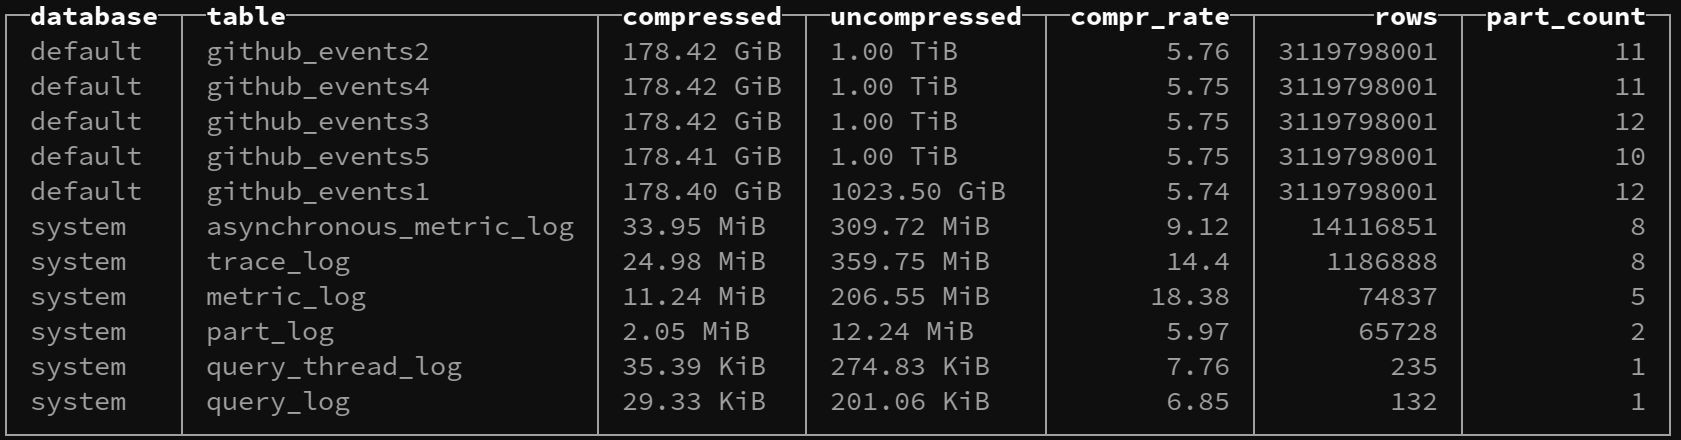
\includegraphics[width=.9\linewidth]{figures/clickhouse/table_sizes.png}
\end{center}
\subsection{Install \texttt{clickhouse-backup}}
\label{sec:org3015272}
The most recent (as of 2022-05-09) \texttt{clickhouse-backup} binary was downloaded
from \texttt{clickhouse-backup}'s GitHub page \cite{akulov_clickhouse-backup_2022}.
%[akulovClickhousebackup2022].

\begin{minted}[breaklines=true,breakanywhere=true]{bash}
# Download archive containing binary
wget https://github.com/AlexAkulov/clickhouse-backup/releases/download/v1.3.2/clickhouse-backup-linux-amd64.tar.gz

# Decompress archive
tar -zxvf clickhouse-backup-linux-amd64.tar.gz

# Move binary to home directory
mv build/linux/amd64/clickhouse-backup ~

# Cleanup
rmdir -p build/linux/amd64
rm clickhouse-backup-linux-amd64.tar.gz
\end{minted}
\subsection{Set up Azure Blob storage for use with \texttt{clickhouse-backup}}
\label{sec:orgf1120ab}
Commands run from the Azure Cloud Shell
\subsubsection{Create a storage account}
\label{sec:org7131bc2}
\begin{minted}[breaklines=true,breakanywhere=true]{powershell}
az storage account create `
    --name $SAName `
    --resource-group $RGName `
    --location eastus `
    --sku Standard_LRS `
    --encryption-services blob
\end{minted}

Output:
\begin{minted}[breaklines=true,breakanywhere=true]{json}
{
  "accessTier": "Hot",
  "allowBlobPublicAccess": true,
  "allowCrossTenantReplication": null,
  "allowSharedKeyAccess": null,
  "allowedCopyScope": null,
  "azureFilesIdentityBasedAuthentication": null,
  "blobRestoreStatus": null,
  "creationTime": "2022-05-10T09:55:00.481299+00:00",
  "customDomain": null,
  "defaultToOAuthAuthentication": null,
  "dnsEndpointType": null,
  "enableHttpsTrafficOnly": true,
  "enableNfsV3": null,
  "encryption": {
    "encryptionIdentity": null,
    "keySource": "Microsoft.Storage",
    "keyVaultProperties": null,
    "requireInfrastructureEncryption": null,
    "services": {
      "blob": {
        "enabled": true,
        "keyType": "Account",
        "lastEnabledTime": "2022-05-10T09:55:00.606291+00:00"
      },
      "file": {
        "enabled": true,
        "keyType": "Account",
        "lastEnabledTime": "2022-05-10T09:55:00.606291+00:00"
      },
      "queue": null,
      "table": null
    }
  },
  "extendedLocation": null,
  "failoverInProgress": null,
  "geoReplicationStats": null,
  "id": "/subscriptions/4b48eb85-91f3-4902-b74b-e84641fb6785/resourceGroups/perfRG/providers/Microsoft.Storage/storageAccounts/perfchbksa",
  "identity": null,
  "immutableStorageWithVersioning": null,
  "isHnsEnabled": null,
  "isLocalUserEnabled": null,
  "isSftpEnabled": null,
  "keyCreationTime": {
    "key1": "2022-05-10T09:55:00.606291+00:00",
    "key2": "2022-05-10T09:55:00.606291+00:00"
  },
  "keyPolicy": null,
  "kind": "StorageV2",
  "largeFileSharesState": null,
  "lastGeoFailoverTime": null,
  "location": "eastus",
  "minimumTlsVersion": "TLS1_0",
  "name": "perfchbksa",
  "networkRuleSet": {
    "bypass": "AzureServices",
    "defaultAction": "Allow",
    "ipRules": [],
    "resourceAccessRules": null,
    "virtualNetworkRules": []
  },
  "primaryEndpoints": {
    "blob": "https://perfchbksa.blob.core.windows.net/",
    "dfs": "https://perfchbksa.dfs.core.windows.net/",
    "file": "https://perfchbksa.file.core.windows.net/",
    "internetEndpoints": null,
    "microsoftEndpoints": null,
    "queue": "https://perfchbksa.queue.core.windows.net/",
    "table": "https://perfchbksa.table.core.windows.net/",
    "web": "https://perfchbksa.z13.web.core.windows.net/"
  },
  "primaryLocation": "eastus",
  "privateEndpointConnections": [],
  "provisioningState": "Succeeded",
  "publicNetworkAccess": null,
  "resourceGroup": "perfRG",
  "routingPreference": null,
  "sasPolicy": null,
  "secondaryEndpoints": null,
  "secondaryLocation": null,
  "sku": {
    "name": "Standard_LRS",
    "tier": "Standard"
  },
  "statusOfPrimary": "available",
  "statusOfSecondary": null,
  "storageAccountSkuConversionStatus": null,
  "tags": {},
  "type": "Microsoft.Storage/storageAccounts"
}
\end{minted}

\subsubsection{Create a storage container}
\label{sec:org80fd248}
\begin{minted}[breaklines=true,breakanywhere=true]{powershell}
az storage container create `
    --account-name $SAName `
    --name $ContainerName `
    --auth-mode login
\end{minted}

Output:
\begin{minted}[breaklines=true,breakanywhere=true]{json}
{
  "created": true
}
\end{minted}
\subsubsection{Enable soft delete for Blobs and Blob container}
\label{sec:org35b84b2}
Enable soft delete for Blob container:
\begin{minted}[breaklines=true,breakanywhere=true]{powershell}
az storage account blob-service-properties update `
    --enable-container-delete-retention true `
    --container-delete-retention-days 7 `
    --account-name $SAName `
    --resource-group $RGName
\end{minted}

Output:
\begin{minted}[breaklines=true,breakanywhere=true]{json}
{
  "automaticSnapshotPolicyEnabled": null,
  "changeFeed": null,
  "containerDeleteRetentionPolicy": {
    "allowPermanentDelete": null,
    "days": 7,
    "enabled": true
  },
  "cors": {
    "corsRules": []
  },
  "defaultServiceVersion": null,
  "deleteRetentionPolicy": {
    "allowPermanentDelete": false,
    "days": null,
    "enabled": false
  },
  "id": "/subscriptions/4b48eb85-91f3-4902-b74b-e84641fb6785/resourceGroups/perfRG/providers/Microsoft.Storage/storageAccounts/perfchbksa/blobServices/default",
  "isVersioningEnabled": null,
  "lastAccessTimeTrackingPolicy": null,
  "name": "default",
  "resourceGroup": "perfRG",
  "restorePolicy": null,
  "sku": null,
  "type": "Microsoft.Storage/storageAccounts/blobServices"
}
\end{minted}

Enable soft delete for all Blobs:
\begin{minted}[breaklines=true,breakanywhere=true]{powershell}
az storage account blob-service-properties update --account-name $SAName `
    --resource-group $RGName `
    --enable-delete-retention true `
    --delete-retention-days 7
\end{minted}

Output:
\begin{minted}[breaklines=true,breakanywhere=true]{json}
{
  "automaticSnapshotPolicyEnabled": null,
  "changeFeed": null,
  "containerDeleteRetentionPolicy": {
    "allowPermanentDelete": null,
    "days": 7,
    "enabled": true
  },
  "cors": {
    "corsRules": []
  },
  "defaultServiceVersion": null,
  "deleteRetentionPolicy": {
    "allowPermanentDelete": null,
    "days": 7,
    "enabled": true
  },
  "id": "/subscriptions/4b48eb85-91f3-4902-b74b-e84641fb6785/resourceGroups/perfRG/providers/Microsoft.Storage/storageAccounts/perfchbksa/blobServices/default",
  "isVersioningEnabled": null,
  "lastAccessTimeTrackingPolicy": null,
  "name": "default",
  "resourceGroup": "perfRG",
  "restorePolicy": null,
  "sku": null,
  "type": "Microsoft.Storage/storageAccounts/blobServices"
}
\end{minted}
\subsection{Configure \texttt{clickhouse-backup} to use Blob storage}
\label{sec:org05c9377}
\subsubsection{Get necessary config details}
\label{sec:org28a9875}
The configuration details needed to configure \texttt{clickhouse-backup} were retrieved
and copied into the configuration file.

Commands were run from the Azure Cloud Shell.

\begin{enumerate}
\item Get access key for storage account
\label{sec:org9369db9}
Get storage account keys:
\begin{minted}[breaklines=true,breakanywhere=true]{powershell}
az storage account keys list `
  --resource-group $RGName `
  --account-name $SAName
\end{minted}

Output:
\begin{minted}[breaklines=true,breakanywhere=true]{json}
[
  {
    "creationTime": "2022-05-10T09:55:00.606291+00:00",
    "keyName": "key1",
    "permissions": "FULL",
    "value": "EIhee0y3zertAVbAa7cRAhYQ/2Oui25vdr6DoL05qkA+CfZZpFMlabzJFPtJG8Xdc735PAbA8w8r+AStl89ieA=="
  },
  {
    "creationTime": "2022-05-10T09:55:00.606291+00:00",
    "keyName": "key2",
    "permissions": "FULL",
    "value": "4Rm6943iYttVqjLBE/csYCa7rnS02xQKjAPW7C/sScZ189My20+/Opl0HmOql1CLnL53x5NYzB/5+AStAqv2kw=="
  }
]
\end{minted}

\texttt{key1} was copied.

\item Get SAS token for container
\label{sec:org2a7114d}
Generate SAS token
\begin{minted}[breaklines=true,breakanywhere=true]{powershell}
az storage container generate-sas `
    --account-name $SAName `
    --name $ContainerName `
    --permissions acdlrw `
    --expiry $SASExpDate `
    --auth-mode login `
    --as-user
\end{minted}

Output:

\begin{minted}[breaklines=true,breakanywhere=true]{text}
"se=2022-05-18&sp=racwdl&sv=2021-04-10&sr=c&skoid=d404139d-e156-421c-9450-19e9734a8141&sktid=09a10672-822f-4467-a5ba-5bb375967c05&skt=2022-05-11T07%3A01%3A18Z&ske=2022-05-18T00%3A00%3A00Z&sks=b&skv=2021-04-10&sig=GgFsZifUWr0r71gCZaD9PbxRXrybhWS09Hpb2scfsKg%3D"
\end{minted}
\end{enumerate}
\subsubsection{Configure \texttt{clickhouse-backup} to use Blob storage}
\label{sec:org265a2b6}
The configuration file from the non-performance test environment
was copied and modified to use the new account key and SAS token.
\texttt{account\_name}, \texttt{container} and \texttt{path} was also modified.
It was saved as \path{/home/azureuser/config.yaml} on the ClickHouse VM.

\begin{minted}[breaklines=true,breakanywhere=true]{yaml}
general:
  remote_storage: azblob
  max_file_size: 0
  disable_progress_bar: false
  backups_to_keep_local: 0
  backups_to_keep_remote: 0
  log_level: info
  allow_empty_backups: false
  download_concurrency: 1
  upload_concurrency: 1
  restore_schema_on_cluster: ""
  upload_by_part: true
  download_by_part: true
clickhouse:
  username: default
  password: ""
  host: localhost
  port: 9000
  disk_mapping: {}
  skip_tables:
  - system.*
  - INFORMATION_SCHEMA.*
  - information_schema.*
  timeout: 5m
  freeze_by_part: false
  secure: false
  skip_verify: false
  sync_replicated_tables: false
  log_sql_queries: true
  config_dir: /etc/clickhouse-server/
  restart_command: systemctl restart clickhouse-server
  ignore_not_exists_error_during_freeze: true
  tls_key: ""
  tls_cert: ""
  tls_ca: ""
  debug: false
s3:
  access_key: ""
  secret_key: ""
  bucket: ""
  endpoint: ""
  region: us-east-1
  acl: private
  assume_role_arn: ""
  force_path_style: false
  path: ""
  disable_ssl: false
  compression_level: 1
  compression_format: tar
  sse: ""
  disable_cert_verification: false
  storage_class: STANDARD
  concurrency: 1
  part_size: 0
  max_parts_count: 10000
  debug: false
gcs:
  credentials_file: ""
  credentials_json: ""
  bucket: ""
  path: ""
  compression_level: 1
  compression_format: tar
  debug: false
  endpoint: ""
cos:
  url: ""
  timeout: 2m
  secret_id: ""
  secret_key: ""
  path: ""
  compression_format: tar
  compression_level: 1
  debug: false
api:
  listen: localhost:7171
  enable_metrics: true
  enable_pprof: false
  username: ""
  password: ""
  secure: false
  certificate_file: ""
  private_key_file: ""
  create_integration_tables: false
  allow_parallel: false
ftp:
  address: ""
  timeout: 2m
  username: ""
  password: ""
  tls: false
  path: ""
  compression_format: tar
  compression_level: 1
  concurrency: 1
  debug: false
sftp:
  address: ""
  port: 22
  username: ""
  password: ""
  key: ""
  path: ""
  compression_format: tar
  compression_level: 1
  concurrency: 1
  debug: false
azblob:
  endpoint_suffix: core.windows.net
  account_name: "perfchbksa"
  account_key: "EIhee0y3zertAVbAa7cRAhYQ/2Oui25vdr6DoL05qkA+CfZZpFMlabzJFPtJG8Xdc735PAbA8w8r+AStl89ieA=="
  sas: "se=2022-05-18&sp=racwdl&sv=2021-04-10&sr=c&skoid=d404139d-e156-421c-9450-19e9734a8141&sktid=09a10672-822f-4467-a5ba-5bb375967c05&skt=2022-05-11T07%3A01%3A18Z&ske=2022-05-18T00%3A00%3A00Z&sks=b&skv=2021-04-10&sig=GgFsZifUWr0r71gCZaD9PbxRXrybhWS09Hpb2scfsKg%3D"
  use_managed_identity: false
  container: "chbkperfcontainer"
  path: "https://perfchbksa.blob.core.windows.net/chbkperfcontainer"
  compression_level: 1
  compression_format: tar
  sse_key: ""
  buffer_size: 0
  buffer_count: 3
  max_parts_count: 1
\end{minted}

\subsubsection{Perform remote backup}
\label{sec:org982a0d7}
Commands were run in \texttt{bash} on the ClickHouse VM.

While the time to \emph{make} backups was not one of the criteria
we decided to focus on, we measured the time anyway.
The time was measured using the builtin bash tool \texttt{time}.
In order to avoid timing \texttt{sudo} the commands were run as \texttt{root}.

Create a remote backup:
\begin{minted}[breaklines=true,breakanywhere=true]{bash}
time ./clickhouse-backup create_remote --config config.yaml
\end{minted}

Time to make a full backup with \texttt{clickhouse-backup}:
\begin{minted}[breaklines=true,breakanywhere=true]{text}
real    198m48.369s
user    14m17.555s
sys     12m38.432s
\end{minted}

List remote backups:
\begin{minted}[breaklines=true,breakanywhere=true]{bash}
./clickhouse-backup list remote --config config.yaml
# 2022/05/11 10:59:53.978855  info SELECT max(toInt64(bytes_on_disk * 1.02)) AS max_file_size FROM system.parts
# 2022-05-11T07-25-16   895.29GiB   11/05/2022 10:44:05   remote      tar
\end{minted}

895GiB is roughly equal to 961GB, which seems correct based on the table sizes.

\subsection{Set up Azure Backup}
\label{sec:org29e551a}
\subsubsection{Create a Recovery Services vault}
\label{sec:orgc6db81c}
\begin{minted}[breaklines=true,breakanywhere=true]{powershell}
az backup vault create --location $location --name $RSVName --resource-group $RGName
\end{minted}

Output:
\begin{minted}[breaklines=true,breakanywhere=true]{json}
{
  "etag": "W/\"datetime'2022-05-10T09%3A58%3A14.2637541Z'\"",
  "id": "/subscriptions/4b48eb85-91f3-4902-b74b-e84641fb6785/resourceGroups/perfRG/providers/Microsoft.RecoveryServices/vaults/perfRSV",
  "identity": null,
  "location": "eastus",
  "name": "perfRSV",
  "properties": {
    "encryption": null,
    "privateEndpointConnections": null,
    "privateEndpointStateForBackup": "None",
    "privateEndpointStateForSiteRecovery": "None",
    "provisioningState": "Succeeded",
    "upgradeDetails": null
  },
  "resourceGroup": "perfRG",
  "sku": {
    "name": "Standard",
    "tier": null
  },
  "systemData": null,
  "tags": null,
  "type": "Microsoft.RecoveryServices/vaults"
}
\end{minted}

\subsubsection{Disable geo-redundancy}
\label{sec:org5e6a978}
\begin{minted}[breaklines=true,breakanywhere=true]{powershell}
az backup vault backup-properties set --backup-storage-redundancy LocallyRedundant --name $RSVName --resource-group $RGName --subscription $subscription
\end{minted}

Output:
\begin{minted}[breaklines=true,breakanywhere=true]{json}
{
  "eTag": null,
  "id": "/subscriptions/4b48eb85-91f3-4902-b74b-e84641fb6785/resourceGroups/perfRG/providers/Microsoft.RecoveryServices/vaults/perfRSV/backupstorageconfig/vaultstorageconfig",
  "location": null,
  "name": "vaultstorageconfig",
  "properties": {
    "crossRegionRestoreFlag": false,
    "dedupState": "Disabled",
    "storageModelType": "LocallyRedundant",
    "storageType": "LocallyRedundant",
    "storageTypeState": "Unlocked",
    "xcoolState": "Disabled"
  },
  "resourceGroup": "perfRG",
  "tags": null,
  "type": "Microsoft.RecoveryServices/vaults/backupstorageconfig"
}
\end{minted}
\subsubsection{Enable backup for the VM}
\label{sec:org6d56370}
\begin{minted}[breaklines=true,breakanywhere=true]{powershell}
az backup protection enable-for-vm `
 --resource-group $RGName `
 --vault-name $RSVName `
 --vm $CHName `
 --policy-name $PolicyName
\end{minted}

Output:
\begin{minted}[breaklines=true,breakanywhere=true]{json}
{
  "eTag": null,
  "id": "/subscriptions/4b48eb85-91f3-4902-b74b-e84641fb6785/resourceGroups/perfRG/providers/Microsoft.RecoveryServices/vaults/perfRSV/backupJobs/e17cce76-2b1e-47e4-a47d-07672d5400cc",
  "location": null,
  "name": "e17cce76-2b1e-47e4-a47d-07672d5400cc",
  "properties": {
    "actionsInfo": null,
    "activityId": "529e46da-d11a-11ec-aebb-0a580af40666",
    "backupManagementType": "AzureIaasVM",
    "containerName": "iaasvmcontainerv2;perfrg;perfclickhousevm",
    "duration": "0:00:30.947098",
    "endTime": "2022-05-11T11:06:30.280573+00:00",
    "entityFriendlyName": "perfclickhousevm",
    "errorDetails": null,
    "extendedInfo": {
      "dynamicErrorMessage": null,
      "estimatedRemainingDuration": null,
      "internalPropertyBag": null,
      "progressPercentage": null,
      "propertyBag": {
        "Policy Name": "DefaultPolicy",
        "VM Name": "perfclickhousevm"
      },
      "tasksList": []
    },
    "isUserTriggered": null,
    "jobType": "AzureIaaSVMJob",
    "operation": "ConfigureBackup",
    "startTime": "2022-05-11T11:05:59.333474+00:00",
    "status": "Completed",
    "virtualMachineVersion": "Compute"
  },
  "resourceGroup": "perfRG",
  "tags": null,
  "type": "Microsoft.RecoveryServices/vaults/backupJobs"
}
\end{minted}

\subsubsection{Make a backup of the ClickHouse VM}
\label{sec:org448ef16}
Instantly trigger a backup job:
\begin{minted}[breaklines=true,breakanywhere=true]{powershell}
az backup protection backup-now `
    --resource-group $RGName `
    --vault-name $RSVName `
    --container-name $CHName `
    --item-name $CHName `
    --backup-management-type AzureIaaSVM `
    --retain-until 18-05-2022
\end{minted}

Output:
\begin{minted}[breaklines=true,breakanywhere=true]{json}
{
  "eTag": null,
  "id": "/subscriptions/4b48eb85-91f3-4902-b74b-e84641fb6785/resourceGroups/perfRG/providers/Microsoft.RecoveryServices/vaults/perfRSV/backupJobs/07a1a270-885a-4210-b7bf-c51f2dcacdad",
  "location": null,
  "name": "07a1a270-885a-4210-b7bf-c51f2dcacdad",
  "properties": {
    "actionsInfo": [
      "1"
    ],
    "activityId": "bb5f9db8-d11a-11ec-8215-0a580af40666",
    "backupManagementType": "AzureIaasVM",
    "containerName": "iaasvmcontainerv2;perfrg;perfclickhousevm",
    "duration": "0:00:01.278993",
    "endTime": null,
    "entityFriendlyName": "perfclickhousevm",
    "errorDetails": null,
    "extendedInfo": {
      "dynamicErrorMessage": null,
      "estimatedRemainingDuration": null,
      "internalPropertyBag": {
        "IsInstantRpJob": "True"
      },
      "progressPercentage": null,
      "propertyBag": {
        "Recovery Point Expiry Time in UTC": "5/18/2022 12:00:00 AM",
        "VM Name": "perfclickhousevm"
      },
      "tasksList": [
        {
          "duration": "0:00:00",
          "endTime": null,
          "instanceId": null,
          "progressPercentage": null,
          "startTime": null,
          "status": "InProgress",
          "taskExecutionDetails": null,
          "taskId": "Take Snapshot"
        },
        {
          "duration": "0:00:00",
          "endTime": null,
          "instanceId": null,
          "progressPercentage": null,
          "startTime": null,
          "status": "NotStarted",
          "taskExecutionDetails": null,
          "taskId": "Transfer data to vault"
        }
      ]
    },
    "isUserTriggered": null,
    "jobType": "AzureIaaSVMJob",
    "operation": "Backup",
    "startTime": "2022-05-11T11:08:52.010975+00:00",
    "status": "InProgress",
    "virtualMachineVersion": "Compute"
  },
  "resourceGroup": "perfRG",
  "tags": null,
  "type": "Microsoft.RecoveryServices/vaults/backupJobs"
}
\end{minted}
\subsubsection{Create a storage account for staging}
\label{sec:orgdb0da58}
A storage account is needed to stage recoveries from Azure Backup.

Create storage account:
\begin{minted}[breaklines=true,breakanywhere=true]{powershell}
az storage account create `
    --name $StagingSAName `
    --resource-group $RGName `
    --location eastus `
    --sku Standard_LRS
\end{minted}

\begin{minted}[breaklines=true,breakanywhere=true]{json}
{
  "accessTier": "Hot",
  "allowBlobPublicAccess": true,
  "allowCrossTenantReplication": null,
  "allowSharedKeyAccess": null,
  "allowedCopyScope": null,
  "azureFilesIdentityBasedAuthentication": null,
  "blobRestoreStatus": null,
  "creationTime": "2022-05-12T06:35:41.131490+00:00",
  "customDomain": null,
  "defaultToOAuthAuthentication": null,
  "dnsEndpointType": null,
  "enableHttpsTrafficOnly": true,
  "enableNfsV3": null,
  "encryption": {
    "encryptionIdentity": null,
    "keySource": "Microsoft.Storage",
    "keyVaultProperties": null,
    "requireInfrastructureEncryption": null,
    "services": {
      "blob": {
        "enabled": true,
        "keyType": "Account",
        "lastEnabledTime": "2022-05-12T06:35:41.272095+00:00"
      },
      "file": {
        "enabled": true,
        "keyType": "Account",
        "lastEnabledTime": "2022-05-12T06:35:41.272095+00:00"
      },
      "queue": null,
      "table": null
    }
  },
  "extendedLocation": null,
  "failoverInProgress": null,
  "geoReplicationStats": null,
  "id": "/subscriptions/4b48eb85-91f3-4902-b74b-e84641fb6785/resourceGroups/perfRG/providers/Microsoft.Storage/storageAccounts/perfstagingchsa",
  "identity": null,
  "immutableStorageWithVersioning": null,
  "isHnsEnabled": null,
  "isLocalUserEnabled": null,
  "isSftpEnabled": null,
  "keyCreationTime": {
    "key1": "2022-05-12T06:35:41.256500+00:00",
    "key2": "2022-05-12T06:35:41.256500+00:00"
  },
  "keyPolicy": null,
  "kind": "StorageV2",
  "largeFileSharesState": null,
  "lastGeoFailoverTime": null,
  "location": "eastus",
  "minimumTlsVersion": "TLS1_0",
  "name": "perfstagingchsa",
  "networkRuleSet": {
    "bypass": "AzureServices",
    "defaultAction": "Allow",
    "ipRules": [],
    "resourceAccessRules": null,
    "virtualNetworkRules": []
  },
  "primaryEndpoints": {
    "blob": "https://perfstagingchsa.blob.core.windows.net/",
    "dfs": "https://perfstagingchsa.dfs.core.windows.net/",
    "file": "https://perfstagingchsa.file.core.windows.net/",
    "internetEndpoints": null,
    "microsoftEndpoints": null,
    "queue": "https://perfstagingchsa.queue.core.windows.net/",
    "table": "https://perfstagingchsa.table.core.windows.net/",
    "web": "https://perfstagingchsa.z13.web.core.windows.net/"
  },
  "primaryLocation": "eastus",
  "privateEndpointConnections": [],
  "provisioningState": "Succeeded",
  "publicNetworkAccess": null,
  "resourceGroup": "perfRG",
  "routingPreference": null,
  "sasPolicy": null,
  "secondaryEndpoints": null,
  "secondaryLocation": null,
  "sku": {
    "name": "Standard_LRS",
    "tier": "Standard"
  },
  "statusOfPrimary": "available",
  "statusOfSecondary": null,
  "storageAccountSkuConversionStatus": null,
  "tags": {},
  "type": "Microsoft.Storage/storageAccounts"
}
\end{minted}
